\documentclass{CSSRforAfrica}

\usepackage[hidelinks,colorlinks=false]{hyperref}
\usepackage{hyperref}
\hypersetup{
    colorlinks=true,
    linkcolor=black,
    filecolor=blue,      
    urlcolor=blue,
    }

\usepackage[titletoc,title]{appendix}
\usepackage{latexsym}
\usepackage{graphicx}
\usepackage{lscape}
\usepackage{pdflscape}
\usepackage{amsmath}
\usepackage[table,dvipsnames,svgnames,x11names]{xcolor}
\usepackage{listings}
\usepackage{tabularx}
\usepackage{forest}
\usepackage{dirtree}
\usepackage{float}
\usepackage{siunitx}
\usepackage{upquote}


\lstset{upquote=true,
        literate={~}{{$\sim$}}1
}
\renewcommand{\DTstyle}{\footnotesize\sffamily}

\definecolor{codegreen}{rgb}{0,0.6,0}
\definecolor{greenyellow}{rgb}{0.8, 0.7, 0.10}
\definecolor{backcolour}{rgb}{0.95,0.95,0.95} 
\definecolor{codepurple}{rgb}{0.58,0,0.82}

\lstdefinestyle{withoutNumbering}{
    backgroundcolor=\color{backcolour},   
    commentstyle=\color{codegreen},
    keywordstyle=\color{magenta},
    stringstyle=\color{codepurple},
    basicstyle=\ttfamily\small,
    breakatwhitespace=false,         
    breaklines=true,                 
    captionpos=b,                    
    keepspaces=true,                 
    showspaces=false,                
    showstringspaces=false,
    showtabs=false,                  
    tabsize=2
}



% the following is added for the note box
\usepackage[most]{tcolorbox}
\newtcolorbox{notebox}[1][]{
  colback=yellow!10!white,
  colframe=black!70!white,
  fonttitle=\bfseries,
  title=NOTE,
  #1
}

\newcommand{\blank}{~\\}
\newcommand{\checkbox}{{~~~~~~~\leavevmode \put(-7,-1.5){  \huge $\Box$  }}}

\begin{document}
\input{epsf}

%%
%% SHOULD NOT NEED TO BE CHANGED BEFORE THIS POINT
%% ------------------------------------------------
%%

\deliverable{D5.5.3}                   % REPLACE with correct number
\title{D5.5.3 Environment Map Generation}        % REPLACE with correct title

\leadpartner{Carnegie Mellon University Africa} % INSERT partner name
\partner{Carnegie Mellon University Africa}     % INSERT partner name

\revision{1.1}                          % REPLACE with correct version number
\deliverabledate{21/03/2025}            % REPLACE with correct date
\submissiondate{04/04/2025}             % REPLACE with correct date
\revisiondate{13/06/2025}                      % REPLACE with date
\disseminationlevel{PU}
\responsible{Birhanu Shimelis Girma}            % REPLACE with correct name

%%
%% Create the titlepage
%%

\maketitle

\section*{Executive Summary}
%===============================================================
\label{executive_summary}

Deliverable D5.5.3 Environment Map Generation focuses on the development of a software module that generates metric workspace and configuration space maps of the environments used in the project's two use case scenarios. These maps include non-symbolic metric data, enabling the Pepper robot to perform path planning and navigate during human-robot interactions. The deliverable focuses primarily on map generation from a priori CAD data.

\noindent The software module, implemented as a ROS node named \texttt{mapGeneration}, produces a map that captures the physical layout of environments using pre-defined geometric data to construct the map. This method generates non-symbolic metric maps visualizable as an image. The module also generates configuration space maps through image dilation, providing essential data for robot navigation planning.

\noindent The development process followed a structured approach that included requirement definition, module specification, implementation, and unit testing. Each phase adhered to the software engineering standards established in Deliverable D3.2, ensuring maintainability and reliability. The configurabiliy of the module through the \texttt{mapGenerationConfiguration.ini} file facilitates its operation in different environments.

\noindent Unit testing confirmed the module's functionality in CAD mode, with tests executed on the physical robot. The tests verified the accuracy of map generation, and the effectiveness of configuration space computation. Overall, this deliverable provides a flexible mapping solution that integrates with other components of the system architecture.



\newpage
\pagebreak
\tableofcontents
\newpage

\section{Introduction}
%===============================================================
This deliverable represents the output of Task 5.5.3, which aims to develop a software module for environment map generation. The module enables the Pepper robot to navigate and make meaningful deictic gestures by providing map that includes physical layout information.

\noindent Environment mapping is a fundamental capability for autonomous robots operating in human-centered spaces. In the context of the CSSR4Africa project, the map serves dual purposes: allowing physical navigation through spaces and supporting meaningful human-robot interaction through references to objects in the environment. The map generation module bridges these requirements by producing a map with metric precision.

\noindent The module supports map generation through a CAD-based approach, which uses a priori data, typically from Computer-Aided Design (CAD) files, to construct the map. The advantage of this method is that it can produce detailed maps without the need for the robot to physically explore the environment. It relies on structured geometric descriptions of the environment to generate workspace and configuration space maps. A workspace map representing the physical environment and a configuration space map derived through image dilation that accounts for the robot's physical dimensions.

\noindent The implementation of the \texttt{mapGeneration} ROS node adheres to the software engineering standards documented in \href{https://cssr4africa.github.io/deliverables/CSSR4Africa_Deliverable_D3.2.pdf}{Deliverable D3.2}. It integrates with other system components, like robot localization, and robot navigation which relies on the generated maps for goal execution. The module's development followed a systematic software engineering process, ensuring maintainability, and integration with the broader system architecture.

\noindent This document details each phase of the development process, from requirements definition through to unit testing, providing a comprehensive overview of the module's functionality, design decisions, and implementation details. The subsequent sections elaborate on the technical aspects of the mapping approach, and the integration with other system components.


\newpage
\section{Requirements Definition}
%===============================================================
The environment map generation module fulfills the functional needs of the users and meets the requirements outlined in the work plan. This section defines the specific requirements that guided the development of the module.

\noindent The module must support map generation using a CAD-based approach with a priori environment data. The generated maps include non-symbolic metric data visualizable as images, and configuration space maps derived through image dilation.

\noindent The configuration space generation functionality converts workspace maps to configuration space maps, applies image dilation using a structuring element modeling the robot's base, and ensures the configuration space accurately represents robot navigability.

\noindent The module supports both the normal operation mode and verbose mode for diagnostics and debugging. In terms of platform compatibility, the module works with both the physical Pepper robot and the Pepper simulator.

\noindent Non-functional requirements include performance specifications, where the module generates maps with sufficient resolution for navigation. Reliability requirements ensure the module generates consistent maps across multiple executions with the same input data, handles edge cases such as basic geometries and overlapping objects, and recovers gracefully from errors in input data. \newline

\noindent The module provides an intuitive interface for map visualization, includes comprehensive error messages for troubleshooting, and supports configurability through parameters. It follows the coding standards outlined in Deliverable D3.2, includes comprehensive internal documentation, and implements modular design for future extensions. Compatibility requirements ensure the module generates maps in formats compatible with ROS navigation stack and supports standard message types for map data.

\newpage
\section{Module Specification}
%===============================================================
The module specification defines the functional capabilities of the environment map generation module, detailing the input to output data transformations, expected input data, output formats, and configuration parameters, as well as the algorithms and data structures used for map generation.

\subsection{Functional Overview}

The \texttt{mapGeneration} module transforms input data from CAD files into a structured representation of the environment with metric information. This transformation includes processing input data to generate a workspace map, applying image dilation to create a configuration space map, saving maps and object data to a file.

\subsection{Input Data Specification}

The module accepts input parameters including map dimensions (width and height in millimeters), obstacle file (containing geometric descriptions of obstacles), parameters file (containing environment parameters), map resolution (meters per pixel), and output filenames for workspace map, and configuration space map.





\subsection{Algorithms and Data Structures}

The CAD-based map generation uses a geometric processing algorithm that parses geometric primitives from the input file, converts to occupancy grid representation, and uses rasterization algorithms for different geometric shapes (Bresenham's \cite{bresenham_algorithm_1965} line algorithm for rectangle edges, flood-fill for interior regions, circle rasterization for circular objects, and polygon filling for complex shapes). \newline

\noindent The configuration space generation uses an image dilation algorithm that converts the occupancy grid to a binary image, defines a structuring element based on robot dimensions (circular element for omnidirectional base, size determined by \texttt{robotRadius} parameter), applies morphological dilation operation, and converts the dilated image back to an occupancy grid. The implementation uses OpenCV for efficient image processing, applies the \texttt{cv::dilate} function with appropriate kernel, and handles edge conditions at map boundaries.


\newpage
\section{Implementation}
%===============================================================
This section details the implementation of the environment map generation module, including file organization, configuration, and core functionality.

\subsection*{File Organization}

The file structure of the map generation module in the \texttt{cssr\_system} package is organized as follows:

\vspace*{0.5em}

\renewcommand*\DTstyle{\ttfamily}
\dirtree{%
.1 cssr\_system.
.2 mapGeneration.
.3 config.
.4 mapGenerationConfiguration.ini.
.3 data.
.4 configurationSpaceMap.png.
.4 environmentMap.png.
.4 mapGenerationInput.dat.
.4 obstacles.dat.
.4 testObstacles.dat.
.3 include.
.4 mapGeneration.
.5 mapGenerationInterface.h.
.3 src.
.4 mapGenerationApplication.cpp.
.4 mapGenerationImplementation.cpp.
.3 README.md.
.3 CMakeLists.txt.
.3 CSSR4AfricaLogo.svg.
}

\subsection*{Configuration Parameters}

\begin{sloppypar}
The operation of the \texttt{mapGeneration} node is determined by the contents 
of a configuration file, \texttt{mapGenerationConfiguration.ini}, that contains 
a list of key-value pairs as shown below in Table \ref{tab:mapGenerationConfiguration.ini}.
\end{sloppypar}

\begin{table}[H]
\centering
\caption{Configuration Parameters for mapGeneration node.}
\label{tab:mapGenerationConfiguration.ini}
\begin{tabular}{|l|l|p{7cm}|}
\hline
\textbf{Key} & \textbf{Values} & \textbf{Effect} \\ \hline
\texttt{mode} & \texttt{CAD, SLAM} & Specifies the map generation approach \\ \hline
\texttt{verboseMode} & \texttt{true, false} & Enables/disables diagnostic output \\ \hline
\texttt{resolution} & decimal value & Specifies map resolution in meters per pixel \\ \hline
\texttt{robotRadius} & decimal value & Specifies the robot base radius \\ \hline
\texttt{inputFile} & string & The input file name \\ \hline
\end{tabular}
\end{table}

\subsection*{Input Files}

For CAD-based map generation, the module requires \texttt{mapGenerationInput.dat} (containing basic parameters including map dimensions, filenames, and resolution), \texttt{obstacles.dat} (defining geometric primitives such as rectangles).

\newpage

\noindent The input files include:

\noindent \texttt{mapGenerationInput.dat}:
\begin{lstlisting}[style=withoutNumbering]
mapWidth 											6.80 # The distance is in meters          			
mapHeight 										9.93							
obstacleFile 									obstacles.dat  			
environmentMapFile 						environmentMap.png 	
configurationSpaceMapFile 		configurationSpaceMap.png   
\end{lstlisting}

\noindent \texttt{obstacles.dat}:
\begin{lstlisting}[style=withoutNumbering]
OBSTACLE   2.57  3.12   2.31 1.44    # Format: TYPE X Y WIDTH HEIGHT
OBSTACLE   1.3   0.45   2.60 0.90
OBSTACLE   2.20  0.30   4.40 0.60
OBSTACLE   3.31  1.925  0.22 0.25
OBSTACLE   3.31  5.525  0.22 0.25
OBSTACLE   3.31  7.325  0.22 0.25
OBSTACLE   3.31  9.125  0.22 0.25
OBSTACLE   0.40  4.965  0.80 9.93
OBSTACLE   3.40  9.465  6.80 0.93
OBSTACLE   6.20  4.965  1.20 9.93

\end{lstlisting}

\subsection*{Output File}
\begin{sloppypar}
The workspace map represents the physical environment in PNG image format and as a ROS OccupancyGrid map representation of free/occupied space, and saved to a file as specified in \texttt{mapGenerationInput.dat}.    
\end{sloppypar}

\begin{sloppypar}
\noindent The configuration space map accounts for robot dimensions, also in PNG image format and as a ROS OccupancyGrid map representation of the robot navigable space, and saved to a file as specified in \texttt{mapGenerationInput.dat}.
\end{sloppypar}


\begin{figure}[H]
  \centering
  % Calculate available space and adjust sizes accordingly
  \begin{minipage}{0.45\textwidth}
    \centering
    
\includegraphics[width=\linewidth,height=6.7cm,keepaspectratio]{images/environmentMap.png}
    \caption{A workspace map representing the physical environment in PNG image format.}
    \label{fig:config_space_map}
  \end{minipage}
  \hfill
  \begin{minipage}{0.45\textwidth}
    \centering
    
\includegraphics[width=\linewidth,height=6.7cm,keepaspectratio]{images/navigationMap.png}
    \caption{A configuration space map accounting for robot dimensions, also in PNG image format and an OccupancyGrid map representation of the robot navigable space.}
    \label{fig:waypoint_map}
  \end{minipage}
\end{figure}

\newpage
\section{Executing Environment Map Generation}
%===============================================================
This section provides a comprehensive guide on setting up, configuring, and executing the \texttt{mapGeneration} node on the physical Pepper robot.

\subsection{Environment Setup}

Before executing the node, several setup steps must be completed to ensure all dependencies are installed and configured correctly. First, all necessary dependencies are installed by navigating to the workspace and running:

\begin{itemize}
\begin{lstlisting}[style=withoutNumbering, language=bash]
cd ~/workspace/pepper_rob_ws
\end{lstlisting}

\begin{lstlisting}[style=withoutNumbering, language=bash]
rosdep install --from-paths src --ignore-src -r -y
\end{lstlisting}

\item If the CSSR4Africa repository has not been cloned yet, this must be done by:
\begin{lstlisting}[style=withoutNumbering, language=bash]
cd ~/workspace/pepper_rob_ws/src
\end{lstlisting}

\begin{lstlisting}[style=withoutNumbering, language=bash]
git clone https://github.com/cssr4africa/cssr4africa.git
\end{lstlisting}

\item Build the package and source the environment:
\begin{lstlisting}[style=withoutNumbering, language=bash]
cd ~/workspace/pepper_rob_ws
\end{lstlisting}
\begin{lstlisting}[style=withoutNumbering, language=bash]
catkin_make
\end{lstlisting}
\begin{lstlisting}[style=withoutNumbering, language=bash]
source devel/setup.bash
\end{lstlisting}

\item Verify the package is correctly placed in the workspace:
\begin{lstlisting}[style=withoutNumbering, language=bash]
ls ~/workspace/pepper_rob_ws/src/cssr4africa/cssr_system/mapGeneration
\end{lstlisting}
\end{itemize}

\begin{figure}[H]
    \centering
    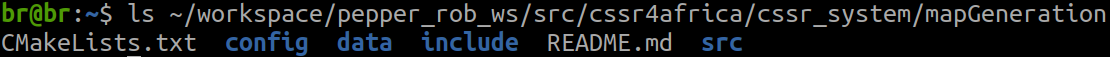
\includegraphics[width=\linewidth]{images/mapGenerationFileDirectory.png}
    \caption{Expected output showing the files and folders in the mapGeneration node}
    \label{fig:map_generation_folder}
\end{figure}

\subsection{Interacting with the Node}

\subsubsection*{Starting the Node}
 It's important to note that the mapGeneration node operates independently of physical robot hardware. You can generate environment maps and configuration space maps without connecting to a Pepper robot. Since the CAD-based map generation relies solely on geometric data provided in input files, no sensor data or robot connectivity is required. Make sure you start a roscore in a new terminal.

\newpage 
\noindent To start the \texttt{mapGeneration} node directly, the following command is used:

\begin{lstlisting}[style=withoutNumbering, language=bash]
rosrun cssr_system mapGeneration
\end{lstlisting}
\begin{figure}[H]
    \centering
    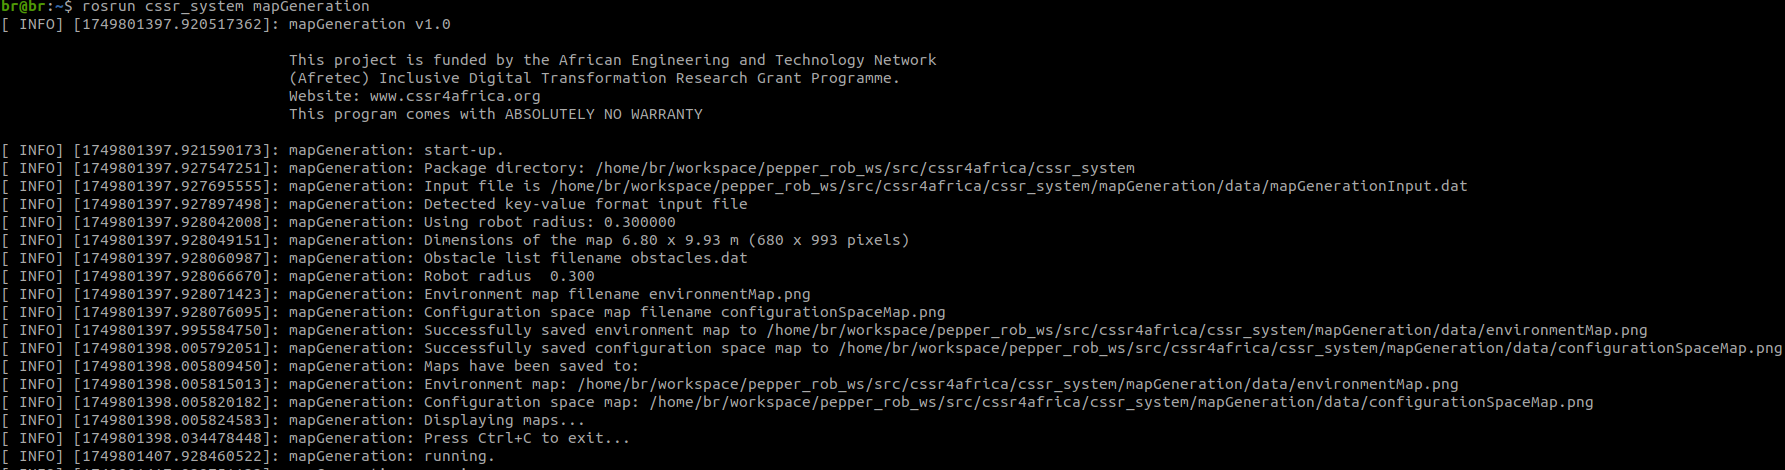
\includegraphics[width=\linewidth]{images/mapGenerationOutput.png}
    \caption{Screenshot of the output of running the mapGeneration node.}
    \label{fig:map_generation_output}
\end{figure}

\subsubsection*{Verifying the Results}

After map generation is complete, the results should be verified by checking that the output files have been created in the specified location \texttt{cssr\_system/mapGeneration/data}, inspecting the workspace map and configuration space map for accuracy.

\newpage

\section{Unit Test}
%===============================================================
Unit testing verifies that the module meets its specifications and functions correctly in various scenarios. This section details the testing approach, setup, and results for the environment map generation test node. 

\noindent It's important to note that the mapGenerationTest node has been designed to operate independently of the physical robot hardware.

\subsection{File Organization and Its Purposes}

The unit tests for the map generation module are organized in the following directory structure:

\vspace*{0.5em}

\renewcommand*\DTstyle{\ttfamily}
\dirtree{%
.1 unit\_tests.
.2 mapGenerationTest.
.3 config.
.4 mapGenerationTestConfiguration.ini.
.4 testConfigLargeRobot.ini.
.4 testConfigSmallRobot.ini.
.4 testConfigVerbose.ini.
.3 data.
.4 environmentMap.png.
.4 mapGenerationInput.dat.
.4 testObstacles.dat.
.4 testOutput.
.5 test\_0.100000\_configurationSpaceMap.png.
.5 test\_0.100000\_environmentMap.png.
.5 test\_0.300000\_configurationSpaceMap.png.
.5 test\_0.300000\_environmentMap.png.
.5 test\_0.500000\_configurationSpaceMap.png.
.5 test\_0.500000\_environmentMap.png.
.5 testOutput.logs.
.4 testRobotRadius.dat.
.3 include.
.4 mapGenerationTest.
.5 mapGenerationInterfaceTest.h.
.3 launch.
.4 mapGenerationLaunchTestHarness.launch.
.3 src.
.4 mapGenerationTestApplication.cpp.
.4 mapGenerationTestImplementation.cpp.
.3 CMakeLists.txt.
.3 README.md.
} 

\noindent The purpose of each file in this structure is to support testing of the map generation node. The configuration files sets test parameters, the data file provides input for the tests, the header file defines interfaces for testing, the source files implement the test cases, and the launch files enable easy execution of tests.

\subsection{Test Environment Setup}

The unit tests are designed to validate CAD-based map generation functionality. Before executing the tests, the testing environment must be properly configured. All necessary dependencies must be installed, the CSSR4Africa repository must be cloned into the workspace if not already present, and the workspace must be built and sourced.

\subsection{Test Cases}

The unit tests are designed to validate specific functionality of the map generation node across different scenarios. Each test case focuses on different aspects of the map generation process. \\

\noindent Test Case 1: Basic CAD Map Generation \\
Tests the core functionality by launching the actual mapGeneration node with standard configuration. Validates that both environment and configuration space maps are generated with correct dimensions and that the configuration space contains more obstacles than the environment map due to robot radius expansion.\\

\noindent Expected Output: A workspace map showing rectangular obstacles as specified in the test\_obstacles.dat file. The resulting map should match the reference image shown in Figure \ref{fig:workspace_map}.\\

\noindent Test Case 2: Configuration Space Generation \\
This test validates the dilation algorithm used to create the configuration space. It tests the generation of configuration spaces with varying robot radii (0.1m, 0.2m, 0.3m, 0.5m, and 0.8m), correct application of structuring elements based on robot dimensions, progressive increase in obstacle area as robot radius increases, and consistent handling of map boundaries during dilation.\\

\noindent Expected Output: Three configuration space maps with progressively larger dilated obstacles, corresponding to the different robot radii. Figure \ref{fig:config_space_0.1m},\ref{fig:config_space_0.3m}, and \ref{fig:config_space_0.5m} shows the comparison between the workspace map and a configuration space map with at a different robot radius.\\

\noindent Test Case 3: Verbose Mode Configuration Test \\
Tests the verboseMode configuration parameter to ensure the node behaves correctly in both interactive (`verboseMode=true`) and automated (`verboseMode=false`) modes.

\begin{figure}[H]
  \centering
  % Workspace map
  \begin{minipage}{0.45\textwidth}
    \centering
    
\includegraphics[width=\linewidth,height=5cm,keepaspectratio]{images/environmentMap.png}
    \caption{Workspace map showing the obstacles on the map in black color.}
    \label{fig:workspace_map}
  \end{minipage}
  \hfill
  % Configuration space map with 0.1m radius
  \begin{minipage}{0.45\textwidth}
    \centering
    
\includegraphics[width=\linewidth,height=5cm,keepaspectratio]{images/configurationMap0.1.png}
    \caption{Configuration space map with 0.1m robot radius}
    \label{fig:config_space_0.1m}
  \end{minipage}
\end{figure}

\begin{figure}[H]
  \centering
  % Configuration space map with 0.3m radius
  \begin{minipage}{0.45\textwidth}
    \centering
    
\includegraphics[width=\linewidth,height=5cm,keepaspectratio]{images/configurationMap0.3.png}
    \caption{Configuration space map with 0.3m robot radius}
    \label{fig:config_space_0.3m}
  \end{minipage}
  \hfill
  % Configuration space map with 0.5m radius
  \begin{minipage}{0.45\textwidth}
    \centering
    
\includegraphics[width=\linewidth,height=5cm,keepaspectratio]{images/configurationMap0.5.png}
    \caption{Configuration space map with 0.5m robot radius}
    \label{fig:config_space_0.5m}
  \end{minipage}
\end{figure}

\noindent Each test case generates both workspace and configuration space maps, which can be found in the test output directory after test execution. The test logs (shown in Appendix I) provide detailed information about each test's execution and verification steps.
\newpage
\subsection{Executing the Map Generation Unit Test}

It's important to note that the mapGenerationTest node has been designed to operate independently of the physical robot hardware. Users can generate environment maps and configuration space maps without needing to connect to a Pepper robot. Since the CAD-based map generation relies solely on geometric data provided in the input files, no sensor data or robot connectivity is required. This makes the node useful for pre-planning environments before deploying the robot, and enables development and testing on any computer with ROS installed and roscore running.

\noindent You can run the test in two ways:

\noindent Using rosrun:
\begin{lstlisting}[style=withoutNumbering, language=bash]
cd $HOME/workspace/pepper_rob_ws
\end{lstlisting}
\begin{lstlisting}[style=withoutNumbering, language=bash]
source devel/setup.bash
\end{lstlisting}
\begin{lstlisting}[style=withoutNumbering, language=bash]
rosrun unit_tests mapGenerationTest
\end{lstlisting}
Using roslaunch (recommended):
\begin{lstlisting}[style=withoutNumbering, language=bash]
roslaunch unit_tests mapGenerationLaunchTestHarness.launch
\end{lstlisting}

\subsection{Test Results}

The results of the unit test confirms that the map generation node meets all specified requirements for CAD-based mapping. The node successfully generates workspace maps, and  computes configuration spaces. Performance is within expected parameters, ensuring the module can operate efficiently in real-world conditions.

\noindent All test cases have passed, indicating that the node functions correctly according to its specifications. Detailed test logs are included in Appendix I, providing a record of all test executions.

\newpage
\appendix

\begin{landscape} 
\section*{Appendix I: Unit Test Logs}
\addcontentsline{toc}{section}{Appendix I: Unit Test Logs}

\small  
\begin{verbatim}
[ INFO] [1749131075]: mapGenerationTest: v1.0 

                      This project is funded by the African Engineering and Technology Network
                      (Afretec) Inclusive Digital Transformation Research Grant Programme.
                      Website: www.cssr4africa.org
                      This program comes with ABSOLUTELY NO WARRANTY

[ INFO] [1749131075]: mapGenerationTest: start-up.

[2025-06-05 15:44:35] mapGenerationTest: =======================================================================
[2025-06-05 15:44:35] mapGenerationTest: === New Map Generation Test Run Started at 2025-06-05 15:44:35 ===
[2025-06-05 15:44:35] mapGenerationTest: =======================================================================
[2025-06-05 15:44:35] mapGenerationTest: Testing Actual Map Generation Node: STARTED
[2025-06-05 15:44:35] mapGenerationTest: -----------------------------------------------------------------------
[2025-06-05 15:44:35] mapGenerationTest: Test Case: MapGenerationTest.BasicMapGeneration
[2025-06-05 15:44:35] mapGenerationTest: Loaded radius1: 0.100000m
[2025-06-05 15:44:35] mapGenerationTest: Loaded radius2: 0.200000m
[2025-06-05 15:44:35] mapGenerationTest: Loaded radius3: 0.300000m
[2025-06-05 15:44:35] mapGenerationTest: Loaded radius4: 0.500000m
[2025-06-05 15:44:35] mapGenerationTest: Loaded radius5: 0.800000m
[2025-06-05 15:44:35] mapGenerationTest: Testing basic map generation with actual mapGeneration node...
[2025-06-05 15:44:35] mapGenerationTest: Launching actual mapGeneration node...
[2025-06-05 15:45:05] mapGenerationTest: [SUCCESS] mapGeneration node completed execution
[2025-06-05 15:45:06] mapGenerationTest: [SUCCESS] Both output maps were created successfully
[2025-06-05 15:45:06] mapGenerationTest: Validating map dimensions...
[2025-06-05 15:45:06] mapGenerationTest: Maps have correct dimensions: 680x993
[2025-06-05 15:45:06] mapGenerationTest: Environment map obstacles: 306011
[2025-06-05 15:45:06] mapGenerationTest: Configuration space obstacles: 444107
[2025-06-05 15:45:06] mapGenerationTest: [SUCCESS] Configuration space correctly has more obstacles than environment map
[2025-06-05 15:45:06] mapGenerationTest: Basic map generation test: PASSED
[2025-06-05 15:45:06] mapGenerationTest: -----------------------------------------------------------------------
[2025-06-05 15:45:06] mapGenerationTest: Test Case: MapGenerationTest.DifferentRobotRadii
[2025-06-05 15:45:06] mapGenerationTest: Loaded radius1: 0.100000m
[2025-06-05 15:45:06] mapGenerationTest: Loaded radius2: 0.200000m
[2025-06-05 15:45:06] mapGenerationTest: Loaded radius3: 0.300000m
[2025-06-05 15:45:06] mapGenerationTest: Loaded radius4: 0.500000m
[2025-06-05 15:45:06] mapGenerationTest: Loaded radius5: 0.800000m
[2025-06-05 15:45:06] mapGenerationTest: Testing different robot radii configurations...
[2025-06-05 15:45:06] mapGenerationTest: Testing with robot radius: 0.100000m
[2025-06-05 15:45:06] mapGenerationTest: Launching actual mapGeneration node...
[2025-06-05 15:45:06] mapGenerationTest: [SUCCESS] mapGeneration node completed execution
[2025-06-05 15:45:07] mapGenerationTest: [SUCCESS] Both output maps were created successfully
[2025-06-05 15:45:07] mapGenerationTest: Validating map dimensions...
[2025-06-05 15:45:07] mapGenerationTest: Maps have correct dimensions: 680x993
[2025-06-05 15:45:07] mapGenerationTest: Environment map obstacles: 306011
[2025-06-05 15:45:07] mapGenerationTest: Configuration space obstacles: 364587
[2025-06-05 15:45:07] mapGenerationTest: [SUCCESS] Configuration space correctly has more obstacles than environment map
[2025-06-05 15:45:07] mapGenerationTest: Robot radius 0.100000m: 364587 obstacle pixels
[2025-06-05 15:45:07] mapGenerationTest: Testing with robot radius: 0.300000m
[2025-06-05 15:45:07] mapGenerationTest: Launching actual mapGeneration node...
[2025-06-05 15:45:07] mapGenerationTest: [SUCCESS] mapGeneration node completed execution
[2025-06-05 15:45:08] mapGenerationTest: [SUCCESS] Both output maps were created successfully
[2025-06-05 15:45:08] mapGenerationTest: Validating map dimensions...
[2025-06-05 15:45:08] mapGenerationTest: Maps have correct dimensions: 680x993
[2025-06-05 15:45:08] mapGenerationTest: Environment map obstacles: 306011
[2025-06-05 15:45:08] mapGenerationTest: Configuration space obstacles: 444107
[2025-06-05 15:45:08] mapGenerationTest: [SUCCESS] Configuration space correctly has more obstacles than environment map
[2025-06-05 15:45:08] mapGenerationTest: Robot radius 0.300000m: 444107 obstacle pixels
[2025-06-05 15:45:08] mapGenerationTest: Testing with robot radius: 0.500000m
[2025-06-05 15:45:08] mapGenerationTest: Launching actual mapGeneration node...
[2025-06-05 15:45:09] mapGenerationTest: [SUCCESS] mapGeneration node completed execution
[2025-06-05 15:45:09] mapGenerationTest: [SUCCESS] Both output maps were created successfully
[2025-06-05 15:45:09] mapGenerationTest: Validating map dimensions...
[2025-06-05 15:45:09] mapGenerationTest: Maps have correct dimensions: 680x993
[2025-06-05 15:45:09] mapGenerationTest: Environment map obstacles: 306011
[2025-06-05 15:45:09] mapGenerationTest: Configuration space obstacles: 518938
[2025-06-05 15:45:09] mapGenerationTest: [SUCCESS] Configuration space correctly has more obstacles than environment map
[2025-06-05 15:45:09] mapGenerationTest: Robot radius 0.500000m: 518938 obstacle pixels
[2025-06-05 15:45:09] mapGenerationTest: Different robot radii test: PASSED
[2025-06-05 15:45:09] mapGenerationTest: -----------------------------------------------------------------------
[2025-06-05 15:45:09] mapGenerationTest: Test Case: MapGenerationTest.VerboseModeTest
[2025-06-05 15:45:09] mapGenerationTest: Loaded radius1: 0.100000m
[2025-06-05 15:45:09] mapGenerationTest: Loaded radius2: 0.200000m
[2025-06-05 15:45:09] mapGenerationTest: Loaded radius3: 0.300000m
[2025-06-05 15:45:09] mapGenerationTest: Loaded radius4: 0.500000m
[2025-06-05 15:45:09] mapGenerationTest: Loaded radius5: 0.800000m
[2025-06-05 15:45:09] mapGenerationTest: Testing verbose mode configuration...
[2025-06-05 15:45:09] mapGenerationTest: Launching actual mapGeneration node...
[2025-06-05 15:45:39] mapGenerationTest: [SUCCESS] mapGeneration node completed execution
[2025-06-05 15:45:40] mapGenerationTest: [SUCCESS] Both output maps were created successfully
[2025-06-05 15:45:40] mapGenerationTest: Validating map dimensions...
[2025-06-05 15:45:40] mapGenerationTest: Maps have correct dimensions: 680x993
[2025-06-05 15:45:40] mapGenerationTest: Environment map obstacles: 306011
[2025-06-05 15:45:40] mapGenerationTest: Configuration space obstacles: 444107
[2025-06-05 15:45:40] mapGenerationTest: [SUCCESS] Configuration space correctly has more obstacles than environment map
[2025-06-05 15:45:40] mapGenerationTest: Verbose mode configuration test: PASSED
[2025-06-05 15:45:40] mapGenerationTest: -----------------------------------------------------------------------
[2025-06-05 15:45:40] mapGenerationTest: =======================================================================
[2025-06-05 15:45:40] mapGenerationTest: === Map Generation Test Run (CAD Mode) Completed at 2025-06-05 15:45:40 ===
[2025-06-05 15:45:40] mapGenerationTest: === All tests PASSED ===
[2025-06-05 15:45:40] mapGenerationTest: =======================================================================
\end{verbatim}
\end{landscape}  

\clearpage

\bibliographystyle{unsrt}
%================================================================
\bibliography{cssr4africa.bib} 
\addcontentsline{toc}{section}{References}

\pagebreak
\section*{Principal Contributors}
%===============================================================
\label{contributors}
\addcontentsline{toc}{section}{Principal Contributors}
The main authors of this deliverable are as follows:
\blank
Birhanu Shimelis Girma, Carnegie Mellon University Africa.\\
David Vernon, Carnegie Mellon University Africa.

\newpage
\section*{Document History}
%================================================================
\addcontentsline{toc}{section}{Document History}
\label{document_history}

\begin{description}

\item [Version 1.0]~\\
First draft. \\
Birhanu Shimelis Girma. \\
04 April 2025.

\item [Version 1.1]~\\
File structure and camel case naming applied to all the file names. \\
Test cases in unit test modified and the output formatting is corrected. \\
Feedback from quality assurance on the software has been updated on the document accordingly.  \\
Birhanu Shimelis Girma. \\
13 June 2025.

\end{description}

\end{document}